%
% File acl2012.tex
%
% Contact: Maggie Li (cswjli@comp.polyu.edu.hk), Michael White (mwhite@ling.osu.edu)
%%
%% Based on the style files for ACL2008 by Joakim Nivre and Noah Smith
%% and that of ACL2010 by Jing-Shin Chang and Philipp Koehn


\documentclass[11pt]{article}
\usepackage{acl2012}
\usepackage{times}
\usepackage{latexsym}
\usepackage{amsmath}
\usepackage{multirow}
\usepackage{url}
\usepackage{graphicx}
\DeclareMathOperator*{\argmax}{arg\,max}
\setlength\titlebox{6.5cm}    % Expanding the titlebox

\title{Instructions for ACL2012 Proceedings}

\author{First Author \\
  Affiliation / Address line 1 \\
  Affiliation / Address line 2 \\
  Affiliation / Address line 3 \\
  {\tt email@domain} \\\And
  Second Author \\
  Affiliation / Address line 1 \\
  Affiliation / Address line 2 \\
  Affiliation / Address line 3 \\
  {\tt email@domain} \\}

\date{}

\begin{document}
\maketitle
\begin{abstract}
  This document contains the instructions for preparing a camera-ready manuscript for the proceedings of ACL2012. The document itself conforms to its own specifications, and is therefore an example of what your manuscript should look like. These instructions should be used for both papers submitted for review and for final versions of accepted papers. Authors are asked to conform to all the directions reported in this document.
\end{abstract}

\section{Introduction}

Crowdsourcing is a promising new mechanism for collecting large volumes of annotated data at low cost.  Platforms like Amazon Mechanical Turk (MTurk) provide researchers with access to large groups of people, who can complete `human intelligence tasks' that are beyond the scope of current artificial intelligence.  Since statistical natural language processing benefits from increased amount of labeled training data, many NLP researchers have focused on creating speech and language data through crowdsourcing (for example,  \newcite{snow2008,callison-burch-dredze2010} and others).  One NLP application that has been the focus of crowdsourced data collection is statistical machine translation (SMT) which requires large bilingual sentence-aligned parallel corpora to train translation models.  Crowdsourcing's low costs has made i possible to hire people to create sufficient volumes of translation in order to train SMT systems.

However, crowdsourcing is not perfect, and one of its most pressing challenges is how to ensure the quality of the data that is created by it.  Unlike more traditional employment mechanism, where our annotator are pre-vetted and their skills are attested for, in crowdsourcing very little is known about the annotators.  They are not professional translators, and their are no built-in mechanisms for testing their language skills.  They complete tasks without any oversight. Thus, translations produced via crowdousrcing may be low quality .
Previous work has addressed this problem, showing that non-professional translators hired on Amazon Mechanical Turk (MTurk) can achieve professional-level quality, by soliciting multiple translations of each source sentence and then choosing the best translation \cite{zaidan-callisonburch:2011:ACL-HLT2011a}.

In this paper we focus on a different aspect of crowdsourcing than \newcite{zaidan-callisonburch:2011:ACL-HLT2011a}.  We attempt to achieve the same high quality while {\bf minimizing the associated costs}.  
%We do so by reducing the number of redundant translations that have to be created for each source segment.   
We  reduce costs using two complementary methods: (1) We quickly identify and filter out workers who produce low quality translations.  The goal is to reduce the number of worker we hire, and retain only high quality translators. 
(2) Instead of soliciting a fixed number of translations for each foreign sentence, we stop soliciting translations after we get an acceptable one.  We do so by building models to distinguish between acceptable translations and unacceptable ones.  The goal is to reduces the number of independent translations that we solicit for each source sentence.
Our work stands in contrast with  \newcite{zaidan-callisonburch:2011:ACL-HLT2011a} who had no model of annotator quality, and who always solicited and paid for a fixed number of translations of each source segment. 
 
 In this paper we demonstrate that
 \begin{itemize}
 \item Workers can be ranked by quality with high correlation against a gold standard ranking ($\rho$ of 0.XXX), using logistic regression and a variety of features, or initially testing them using a small amount of calibration data with known professional translations.
 \item This ranking can be established after observing very small amounts of data (reaching $\rho$ of 0.XXX after seeing only 10 translations from each worker), so bad workers can be filtered out quickly.
 \item Our models can predict whether a given translation is acceptable with high accuracy, subtantially reducing the number of redundant translations needed for every source segment.
 \item We can achieve a similar BLEU score as \newcite{zaidan-callisonburch:2011:ACL-HLT2011a} at $\frac{1}{X}$ of the cost.  
 \end{itemize} 
 
 % This part we might move to a different section.
% For the first approach, we propose several ranking methods to rank workers and to to evaluate their competency. 
%We evaluate workers' competency in several ways: first, we estimate their average quality using all of their translations, then we limit ourselves to the first k-translations that they provide. If we are able to quickly distinguish between high quality versus low quality translators, then we can reduce costs by only soliciting translations from high quality translators.   
%For the second approach, we propose a framework to search for the threshold to separate acceptable and unacceptable translations and judge for a  
%%Also need to mention another work to reduce cost

\section{Cost Optimization}

There are two approaches that we use to reduce costs. In the first approach, we attempt to quickly rank workers and discard low ranking workers. In the second approach, we reduce the number of translations that we buy for each foreign sentence. After receiving a translation, we decide whether its quality is sufficient or whether we ought to pay for another translation (with the hope that the subsequent translation will be better).  In both cases we aim to reduce costs, while keeping our overall translation quality high.
 
 For the first approach, as mentioned in section~\ref{dataanaly}, we show we are able to rank workers accurately using only the translations of their first 4 HITs.  The ranked list of workers using 4 HITs is  almost identical to the gold standard ranking that uses all HITs. In other words, we can predict workers' performance reasonably well, as long as we have obtained a small number of HITs from them.  (Assuming that we have professional translations of their initial HITs, which we can use to calculate their translation quality). Consequently, we can decide whether to continue to hire a worker in a very short time after analyzing the first HIT(s) provided by each worker.
 
 For the second approach,  we train a model to decide whether a translation  is `good enough,' in which case we don't need to  pay for another redundant translation of the source sentence.  To perform this experiment, we divide the data into 3 parts: 10$\%$ of the data as a training set, 10$\%$ of the data as a validation set and the remaining 80$\%$ of the data as a test set. We train the model to score each translation we've got already, to use this score to evaluate whether to get another translation. The challenge is how to set the threshold to separate acceptable translations and unacceptable ones. 
 
 
% Maybe first describe the model features, and then describe how you set the threshold value. 
 In our design, we set the threshold empirically using the validation set after we have trained the model on the disjoint training set. More specifically, during the training process, we get the lower bound and upper bound of scores for translations in the training set. Then we search for the threshold through traversing from the lower bound to the upper bound by a small step size. %add a figure to illustrate the traversal
 We use each value  in the process  as the potential threshold.  We score translations of the foreign sentences in the validation set.  Since this approach assumes a temporal ordering of the translations, we compute the scores for each translation of a source sentence using the time-ordering of when Turkers submitted them. There are 2 conditions on the halt of this process for each foreign sentence: 1) the predicted BLEU score of some translation (submitted earlier than the last translation) is higher than the threshold or 2) we have scored all 4 translations.  

To evaluate the performance of the model running with different thresholds, we first compute an upper bound by selecting the best translation among all 4 candidates for each foreign sentence of the validation set according to our  model. We call this set $S_{upper}$.  $S_{upper}$ is the highest BLEU score we can get by choosing translation using the model, since it has access to all of the available translations.  

After we have used the validation set to sweep various threshold values,  we can pick a suitable value for the threshold by picking the lowest value that is within some delta of $S_{upper}$, say  90$\%$. 

Finally, we retrain our model using the union set of the training set and validation set, use the resulting model on the test set.  We evaluate the model's performance by counting the average number of candidate translations that it solicits per source sentence, and by computing the loss in overall BLEU score compared to when it had access to all 4 translations.  This evaluation shows how much money our model would save by eliminating unnecessary redundancy in the translation process, and how close it is to the upper bound on translation quality when using all of the translations from the original set.


\section{Data}
\subsection{Data Collection}

We use the data collected by  \newcite{zaidan-callisonburch:2011:ACL-HLT2011a} through Amazon's Mechanical Turk(MTurk). MTurk is an online platform provided to people for completing Human Intelligence Tasks(HIT) with a relatively low cost. We use their Urdu-to-English 2009 NIST Evaluation Set as our corpus.  \newcite{zaidan-callisonburch:2011:ACL-HLT2011a}  translated the Urdu side to English through MTurk. They collected the translations in the unit of Human Intelligence Tasks(or HITs). In every HIT, they posted 10 Urdu sentences to be translated. Every sentence is translated by 4 workers, and subsequently post-edited by 10 additional workers.\footnote{\newcite{zaidan-callisonburch:2011:ACL-HLT2011a}  collected their translations in two batches.  The first batch contained 1 translation, each with 1 post-edited  version.  The second contained an additional 3 translations, each of which was post-edited by 3 workers.}
This data set also has four corresponding professional translations for each  of the Urdu sentences, collected by LDC. This makes it possible to compare the Turkers' translation quality to professionals. 

\subsection{Feature Extraction}

Following \newcite{zaidan-callisonburch:2011:ACL-HLT2011a}, we extract a number of features from the translations and workers' self-reported language skills.  We use these to build feature vectors used in tuning model and choosing the best translations from the candidates. 
POTENTIALLY: We extend \newcite{zaidan-callisonburch:2011:ACL-HLT2011a}'s feature set to include additional bilingual features, which were not part of that original work.
\subsubsection*{Sentence-Level Features (9 Features)}
This feature set contains language based features to solely implicate the quality of an English sentence without any suggestion on the bond of the meaning between the source sentence and the translation . This set of features tells good English sentences apart bad ones. The reason we use this set of features is that a good English sentence is the prerequisite of being a good English translation.
\begin{itemize}
\item Language model features:	we assign a log probability and a per-word perplexity score for each sentence. We use SRILM toolkit to calculate perplexity score for each sentence based on 5-gram language model trained on English Gigaword corpus.
\item Sentence length features:	we use the ratio of the length of the Urdu source sentence to the length of  the translation sentence as feature since a good translation is expected to be comparable in length with source sentence. We add two such ratio features( one is designed for unreasonably short translation and the other is for unreasonably long translation).
\item Web \textit{n}-gram log probability feature: we add the Web \textit{n}-gram log probability feature to reflect  the probability of the \textit{n}-grams(up to length 5) exist in the Microsoft Web N-Gram Corpus. For short sentences whose length is less than 5, we use the sentence length as the order of the \textit{n}-gram in calculation.
\item Web \textit{n}-gram geometric average features: we calculate the geometric average \textit{n}-gram  to evaluate the average matching over different \textit{n}-grams. We add 3 features correspondent to max \textit{n}-gram length of 3,4 and 5. Specifically, $P_i$ denotes the log probability of \textit{i}-gram and these 3 features are represented in $\sqrt[3]{P_1 P_2 P_3}$ ,$\sqrt[4]{P_1 P_2 P_3 P_4}$ and $\sqrt[5]{P_1 P_2 P_3 P_4 P_5}$ .
\item Edit rate to other translations: In posterior methods, to minimize Bayes risk, we choose the translation  that is most similar to other translations. Taking this into consideration, we add the edit rate feature to implement the similarity among all candidates translations.
\end{itemize}
 \subsubsection*{Worker-Level Features (15 Features)}
 We take the quality of workers into consideration and add worker level features since the intuition that good workers can always high quality translations.
\begin{itemize}
\item	Aggregate features:	for each sentence level feature, we use the average values over all translations provided by the same worker as that worker's aggregate feature values.
\item	Language abilities:	we collect worker's language ability information about whether the worker is a native Urdu speaker or native English speaker and how long they have spoken English or Urdu and add four features correspondent to the four aspects above.
\item	Worker Location:	we add two features to indicate whether a worker is located in Pakistan or India.
\end{itemize}
 \subsubsection*{Ranking Features (3 Features)}
 \newcite{zaidan-callisonburch:2011:ACL-HLT2011a} collected 5 ranking labels for each translation and refine 3 features from these labels.
 \begin{itemize}
 \item Average Ranking:	the average of the 5 ranking labels for this translation.
 \item Is-Best percentage: this feature shows how often a translation is ranked as the best translation among all candidates translation.
 \item Is-Better percentage: how often a translation is ranked as a better translation based on the pairwise comparisons.
 \end{itemize}
 \subsubsection*{Calibration Feature (1 Feature)}
 We use the average BLEU score of  translations provided by the same worker  as  the calibration feature.
  The BLEU score is computed against references. 
  \subsubsection*{Word Alignment Feature (1 Feature)}
  We 

\subsection{Data Analysis} \label{dataanaly}

We analyze the data considering the timing information that accompanies the translations that we collected. In this analysis, we'd like to evaluate the performance of each worker as time goes on. Each worker translates one or more HITs. Since the translations were collected in two batches, which started at different times, we assign a relative time to each assignment to simulate what would have happened if both batches were run at the same time.  For each HIT, we assign it a relative time by calculating difference between the HIT's submission time and the HIT's creation time. This gives the HIT's relative submission time.  For each worker, we calculated the BLEU score for each of their HITs and analyze the translation quality of the worker at different time points. We are interested in seeing whether workers produce consistently good translations over time or if their quality drops off over time, and if workers who produce bad translations submit them more quickly than workers who submit good translations.  Figure~\ref{fworkerperf} illustrates workers' translation quality at across time. In this graph, each tick represent a single translation HIT, and depicts the HIT's BLEU score (color) and its size/number of sentences (thickness).  The worker who provided the translation is graphed on the y axis, and the submission time is plotted on the x axis. We set the median of all HITs' BLEU scores as the threshold. If the HIT's BLEU score is higher than the median, then the HIT's color is dark.  A light colored tick mark means the HIT's BLEU score is lower than the median. In Figure~\ref{fworkerperf}, the order of workers on y axis is based on the gold standard ranking of these workers. The top most worker ranked highest and the bottom most worker ranked lowest. 

From Figure~\ref{fworkerperf}, we see that most workers' performance stays
consistent as time passes. This is good, since it may enable us to predict workers' performance based on their early submission so that we can come to an early decision about whether to continue to hire them.  If we rank the worker based solely on their first HITs' BLEU score, comparing all sentences in that HIT against the reference translation, then we get a surprisingly strong correlation with the true gold standard ranking of workers based on all of their submitted work. The Spearman Correlation is 0.86 when comparing this first-HIT ranking with gold standard ranking.
\begin{figure}[htbp]
  \centering
  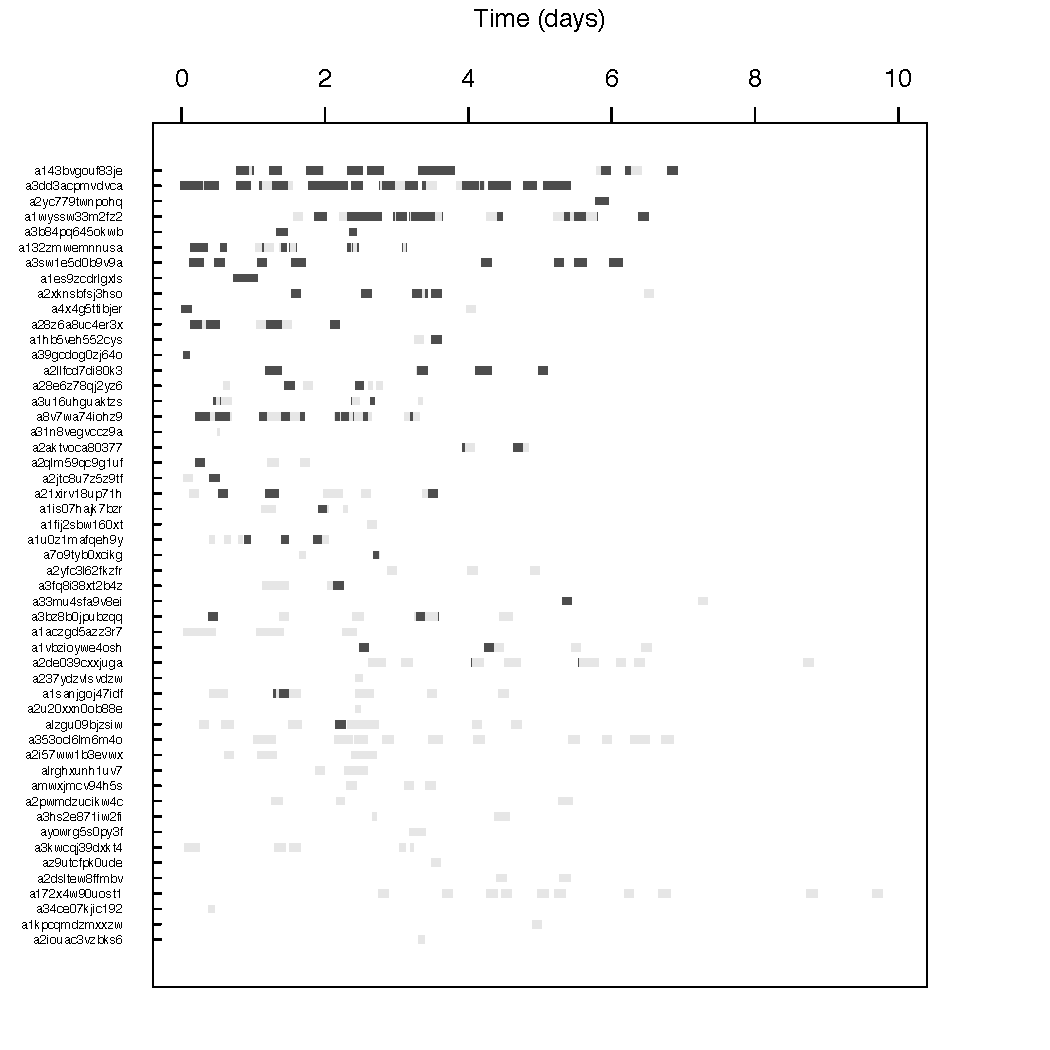
\includegraphics[width=\linewidth]{WorkerPerf/workerperform.pdf}
  \caption{Workers' performance  at across time.}
    \label{fworkerperf}
\end{figure}

Expanding the experiment mentioned above, we rank workers using their first $k$ HITs and calculate Spearman Correlation comparing against the gold standard ranking list (calculated over all HITs, instead of just the first $k$). The value of $k$ could range from 1 to the max number of HITs submitted by any single worker. Since some workers only translated a small number of HITs, larger values of $k$ will be greater than the total number of HITs that they provided. For those workers who translated less than $k$ HITs in total, we use all of the HITs they submitted to rate them.  Since the correlation converges to 1 after $k$ is larger than 10, we plot the graph to show the increase in correlation for $k$ from  1 to 10. Figure~\ref{fcorr} shows details.  The average number HITs each worker provided is 15.06, so we also plot Figure~\ref{fcorrnor} to show the percentage of HITs we use to rank workers for each value of $k$.

    

\begin{figure}[htbp]
  \centering
  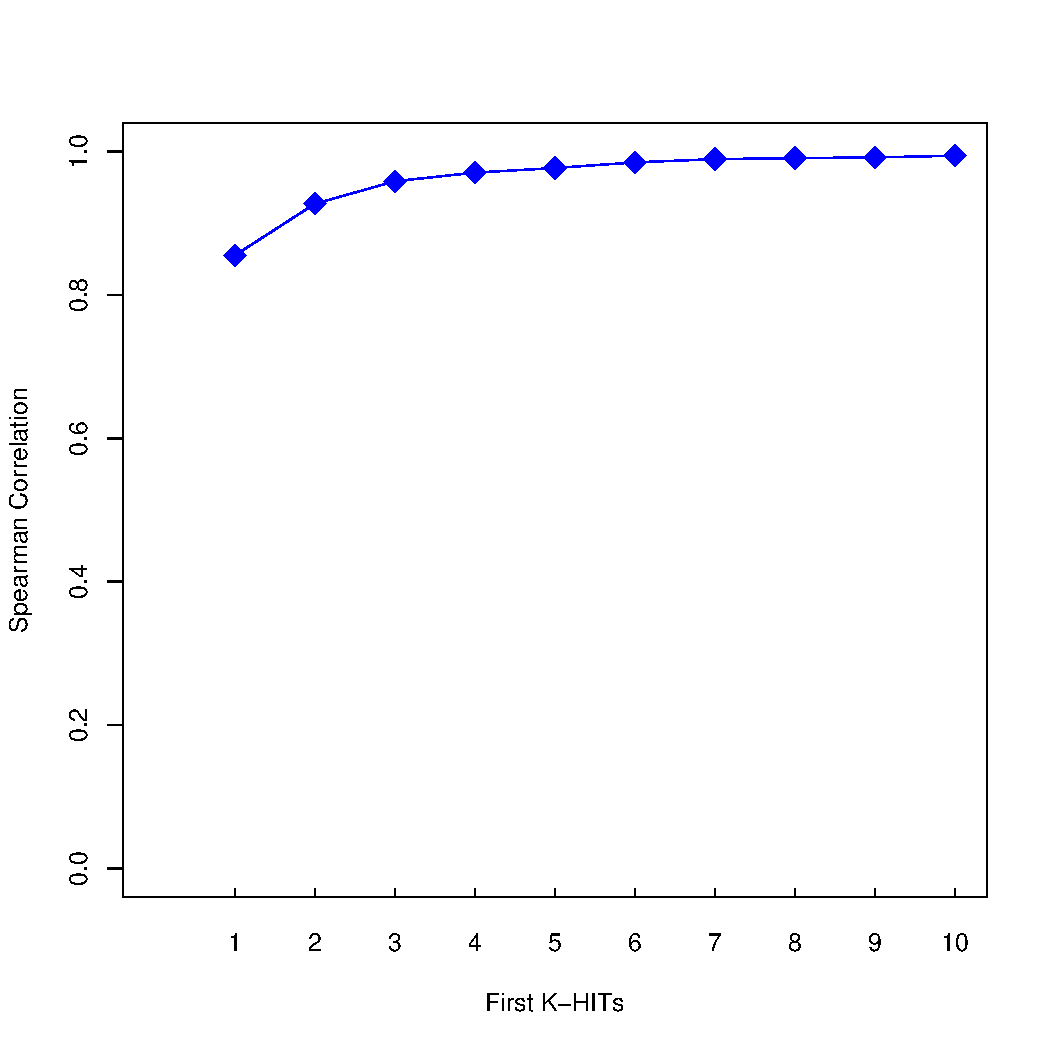
\includegraphics[width=\linewidth]{WorkerPerf/corr.pdf}
  \caption{Spearman Correlation with the gold standard as we rank the workers based on their first $k$ HITs}
    \label{fcorr}
\end{figure}

\begin{figure}[htbp]
  \centering
  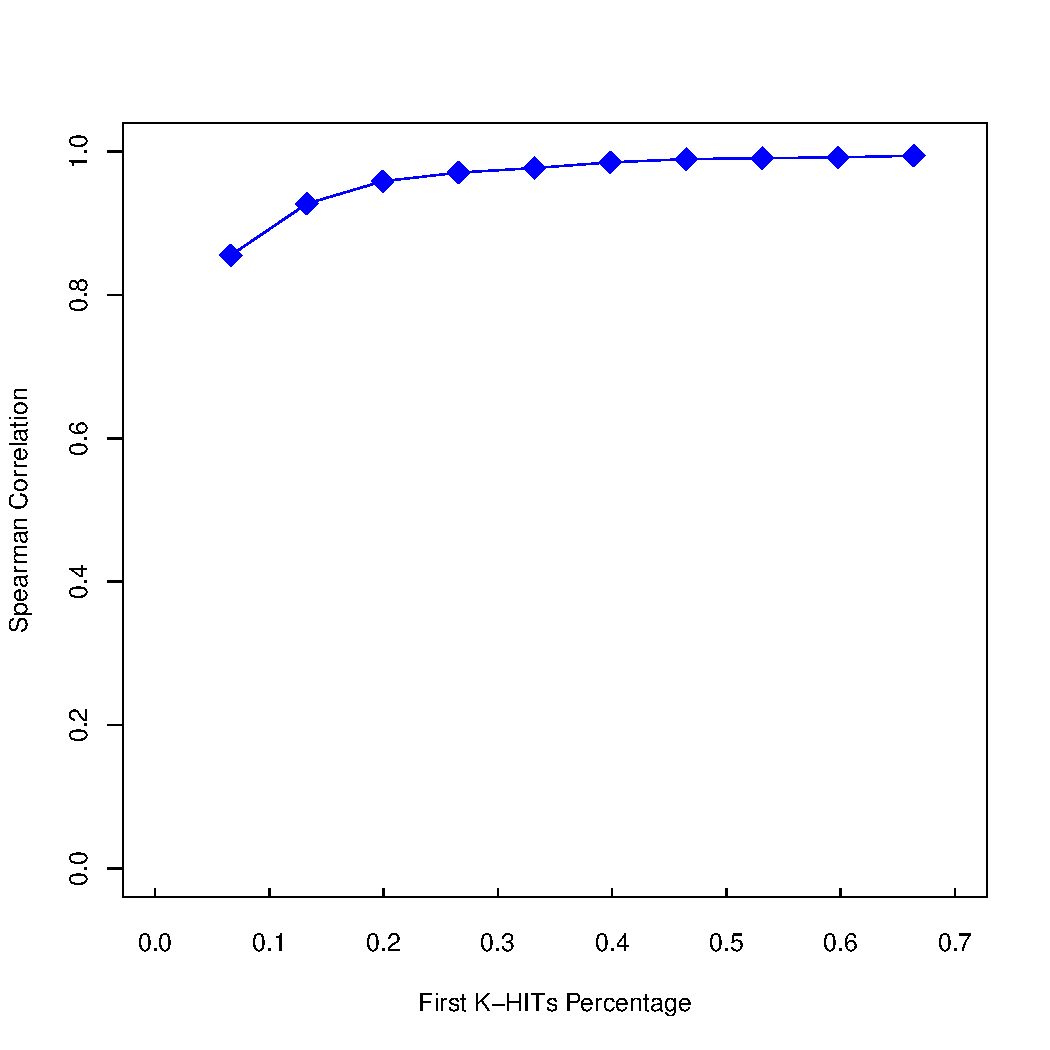
\includegraphics[width=\linewidth]{WorkerPerf/corrnormalized.pdf}
  \caption{The percentage of worker data used to rank them as $k$ increases}
    \label{fcorrnor}
\end{figure}


\section{Experiment}
\section{Related Work}

For one of our approaches for lowering the costs of crowdsourcing,  we train models to distinguish between acceptable and unacceptable translation candidates.  To do so,
% Candidates with BLEU scores higher than the threshold are acceptable and vice versa. We search for the threshold on the validating set that is leading to the BLEU within some delta of $S_{upper}$.  
we sweep a threshold of BLEU values. The threshold between acceptable and unacceptable translations is fuzzy so there exists some uncertainty in labeling each data sample.  This is related to \cite{sheng2008get}'s work on repeated labeling, which presents a way of solving the problems of   uncertainty in labeling and selection of a threshold. In their work, they showed that for single-labeling examples, the labeling quality (the annotator's probability of producing a correct labeling) is critical to the model quality. The model prediction accuracy rises as the labeling quality increases. However, in reality, we cannot always get high-quality labeled data samples with relatively low costs. To keep the model trained on noisy labeled data having a high accuracy in predicting, \newcite{sheng2008get} proposed a framework for repeated-labeling that resolves the uncertainty in labeling via majority voting.  
The experimental results show that a model's predicting accuracy is improved even if labels in its training data are nosity and of imperfect quality.  As long as the integrated quality (the probability of the integrated labeling being correct) is higher than 0.5, repeated labeling benefits model training. More closer the quality to 0.5, the more benefits obtained in model prediction.

%If we relax the condition on the uniform labeler quality and allow lablers to have different quality,  a new question arises: should we use the best individual labeler or should we combile the results from multiple labelers? According to the analysis,  it depends on how much the best labeler's quality is better the average quality of all labelers.

%Majority voting is an useful approach to improve the quality of corpus. However, it omits  the uncertain property of data samples' labels and loses the information about uncertainty in labels. To take advantage of the uncertainty, \newcite{sheng2008get} represent labeling uncertainty in probability. For each unlabeled data sample $x_{i}$, the \textit{multiplied examples} (ME) procedure takes the existing multi-label set  $L_i = \{y_{ij}\}$ as input, and for each label value $y_{ij} $ in the multiset, make a replica of $x_i$ which is labeled $y_{ij}$, and use the probability of that label value appearing in the multi-label set as the weight of that replica . We can use cost-sensitive learning method to train model on the modified data set. Experiment shows that ME strategy is better than than majority voting.

%In experiments, for each data set, 30\% data samples are held out as the test data, and the rest data is the "pool" from which we acquire unlabeled and labeled samples. When deciding the next data sample to be labeled, they use the generalized round robin strategy: selecting the data sample with the fewest labels. To make the selection more reasonable, they proposed the selective-repeated labeling method. For each data sample, $LU$ is defined as the label uncertainty which measures the labels' diversity on the data sample. Similarly, $MU$ is defined as the model uncertainty which measures the disagreement on models' prediction to the data sample. $LMU$ is defined as the label and model uncertainty which is the geometric average of $LU$ and $MU$. Instead of assigning the new label to  the data sample with fewest labels, they choose the data sample with the highest $LMU$ score and get benefits.

%Outline of related work of 'Benefits of a Model of Annotation'.\\
%1. Related Point: our work is trying to find the best translation from all candidates. Their work is trying to %select a label from the multi-label set.
%2. Different Point: our work is don't have labels but they have.

A very important issue in natural language processing is data annotation. Hiring professional annotators is very expensive. As an alternative, collecting several annotation for each single data sample and pick the best label is  more economical.  In our work, we collected several translations for each source sentence and pick the best translation. Our work shares many goals in common with \newcite{passonneau2013benefits}, who created a Bayesian model of annotation, which they applied to the problem of word sense annotation. Rather than hiring professional annotators, which is very expensive, they hire non-expert annotators on Mechanical Turk.  They collected 20 to 25 word sense labels for each word. To decide which label to select for each word, and to compute the quality of the annotation, they proposed the probabilistic model using Bayes's rule. They calculated the product of the prior probability (the initial probability of being the observed label) and the conditional probability (the probability of being the observed label given the true label) and pick one label with the highest score. This sort of a probability estimate provides much more information about the corpus quality than previous methods, such as calculating inter-annotation agreement through Coehn's kappa score.  Kappa measures the agreement coefficient among annotators in a chance-adjusted fashion.  However, the method  only  reports how often annotators agree, but does not provide information about the quality of the corpus and the individual data sample.

Although \newcite{passonneau2013benefits} collect word sense labels, which are a small, enumerable set, and we collect translation (which could be thought of as a kind of label, albeit a very complex one), there is a strong commonality in the goals of their word and the goals of our work.  Specifically, how can we use all the labels collected in order to select of the best label.  And how can we rank the annotators themselves.  For selecting the best label for word senses, majority voting is a direct and easy way to solve the problem, but the task is more complex for translation. 

\newcite{passonneau2013benefits} also proposed an approach to detect and avoid spam workers. 
%They required workers to finish 20000 HITs and have a 98\% lifetime approval rating. 
They measured the performance of worker by comparing worker's labels to the current majority labels and worker with bad performance would be blocked. However, this approach suffered from 2 shortcomings: (1) Sometimes majority labels may not reflect the ground truth label. (2) They didn't figure out  how much data(HITs) is needed to evaluate a worker's performance. Although they could find the spam after the fact, it was a post-hoc analysis, so they had already paid for that worker and wasted the money.  We attempt to identify poor workers as quickly as possible, in order to limit the amount of work that we solicit from them.

\section{Discussion}
\section{Conclusion}
\section*{Acknowledgments}

Do not number the acknowledgment section. Do not include this section when submitting your paper for review.

\bibliographystyle{acl2012}
\bibliography{tacl.bib}

\end{document}